\section{Enclosure Membership and the Visual Model}\label{sec:coord0-enclosures}

\subsection{Even enclosure sequence and cumulative boundaries}\label{subsec:coord0-grouping-derivation}
\paragraph{Setup.}
The inherited enclosure grammar distinguishes \(E_2\) (duon), its open and seated states \(E_2^0,E_2^\pm\), the inner \(E_4\) tetron, and outer even support enclosures \(\mathsf C_{2m}\), \(m\ge3\). The present chart uses \(\mathsf C_6\) through \(\mathsf C_{22}\) as nested enclosure interfaces. Their displayed geometry represents declared enclosure membership; no measured radius or metric scale is assigned. The semantic sources are \mainsection{sec:seat-shell-enclosure-routing} and \mainappendix{app:cc-support-enclosure-names}.

\paragraph{Derivation.}
The coord-0 declaration and filled boundary form are
\begin{equation}
0\mid-::Z:A:0:L\langle a:b:c::L\rangle,
\label{eq:matter1-coord0-declaration}
\end{equation}
\begin{equation}
0\mid-::Z:A:0:2m\langle m:m:0::2m\rangle.
\label{eq:matter1-filled-shared-enclosure}
\end{equation}
Following \mainsection{subsec:coord-zero-support-enclosure-grouping},
\begin{equation}
\Gamma_m=\sum_{k=3}^{m}2k=m(m+1)-6,\qquad \Gamma_2=0,
\label{eq:matter1-gamma-m}
\end{equation}
and
\begin{equation}
\Gamma_{m-1}<Z\le\Gamma_m,\qquad s=Z-\Gamma_{m-1}
\label{eq:matter1-group-selection}
\end{equation}
select the unique group and seat. Here \(Z=1,\ldots,118\) identifies the labelled elements; integers 119--126 are unfilled reference-slot indices in the same grouping.

The local tuple is
\begin{equation}
a(s)=\left\lceil s/2\right\rceil,\qquad
b(s)=\left\lfloor s/2\right\rfloor,\qquad c(s)=s\bmod2.
\label{eq:matter1-seat-abc}
\end{equation}
Thus \(c=1\) records odd local parity and \(c=0\) even local parity. It does not determine an assigned acceptor, neutral or shedding class. For example, Li has \(s=3,c=1\) but an assigned neutral class; O has \(s=2,c=0\) but an assigned acceptor class. The tuple and those input classifications are distinct relations.

\paragraph{Specialization.}
The nine groups in \tabref{tab:matter1-enclosure-groups} contain 126 reference slots, of which 118 carry element labels:
\[
118/126=59/63,\qquad
N_{\mathrm{labelled}}(\mathsf C_{22})/22=14/22=7/11.
\]
These are labelled-reference occupancy fractions. No retention duration or physical limit beyond 118 follows from them.

\begin{table}[H]
\centering
\small
\setlength{\tabcolsep}{4pt}
\caption{\textbf{Declared enclosure groups and local role positions.} The last endpoint is an unfilled reference slot.}
\label{tab:matter1-enclosure-groups}
\begin{tabular}{@{}rrrrlll@{}}
\toprule
\(m\) & \(2m\) & \(\Gamma_{m-1}\) & \(\Gamma_m\) & Index range & Hinge \(s=m\) & Boundary \(s=2m\)\\
\midrule
3 & 6 & 0 & 6 & 1--6 & 3 Li & 6 C\\
4 & 8 & 6 & 14 & 7--14 & 10 Ne & 14 Si\\
5 & 10 & 14 & 24 & 15--24 & 19 K & 24 Cr\\
6 & 12 & 24 & 36 & 25--36 & 30 Zn & 36 Kr\\
7 & 14 & 36 & 50 & 37--50 & 43 Tc & 50 Sn\\
8 & 16 & 50 & 66 & 51--66 & 58 Ce & 66 Dy\\
9 & 18 & 66 & 84 & 67--84 & 75 Re & 84 Po\\
10 & 20 & 84 & 104 & 85--104 & 94 Pu & 104 Rf\\
11 & 22 & 104 & 126 & 105--126 & 115 Mc & 126 --\\
\bottomrule
\end{tabular}
\end{table}

\subsection{Relations before layout}\label{subsec:matter1-visual-model}
\paragraph{Setup.}
The visual model preserves the mapping \(Z\mapsto(m,s,a,b,c)\). Within each enclosure the declared role projection assigns \(1\le s<m\) to the first branch, \(s=m\) to the hinge, \(m<s<2m\) to the counterbranch, and \(s=2m\) to the filled-tuple boundary position. This repeating organization expresses the inherited motif without supplying an executed inter-element edge.

\paragraph{Derivation.}
Nested outlines express enclosure membership; label positions express local order and role. A guide through consecutive seats is an index-order guide. A spiral may project that order while preserving membership, but its curvature is not a temporal trajectory or a transition witness. Assigned classes, when displayed in the companion or table, retain their assigned-input meaning from \secref{sec:fusion-contact-ledger}.

\paragraph{Falsification.}
Changing a preserved \(Z,m,s\) placement, confusing odd parity with an assigned acceptor state, or treating the eight unfilled slots as demonstrated physical non-retention contradicts the declared visual model. Field count \(n_F\log n_F\) in \mainequation{eq:field-count-term} is a different scoped construction; a ring count cannot serve as its field-family witness.

\aodprovenance{\mainsection{subsec:filled-shared-enclosures}, \mainsection{subsec:coord-zero-support-enclosure-grouping}, \mainsection{sec:shell-paths}, \mainsection{subsec:support-enclosure-retention-condition}, \eqnref{eq:matter1-group-selection}, \eqnref{eq:matter1-seat-abc}.}

\begin{figure}[p]
\centering
\makebox[\textwidth][c]{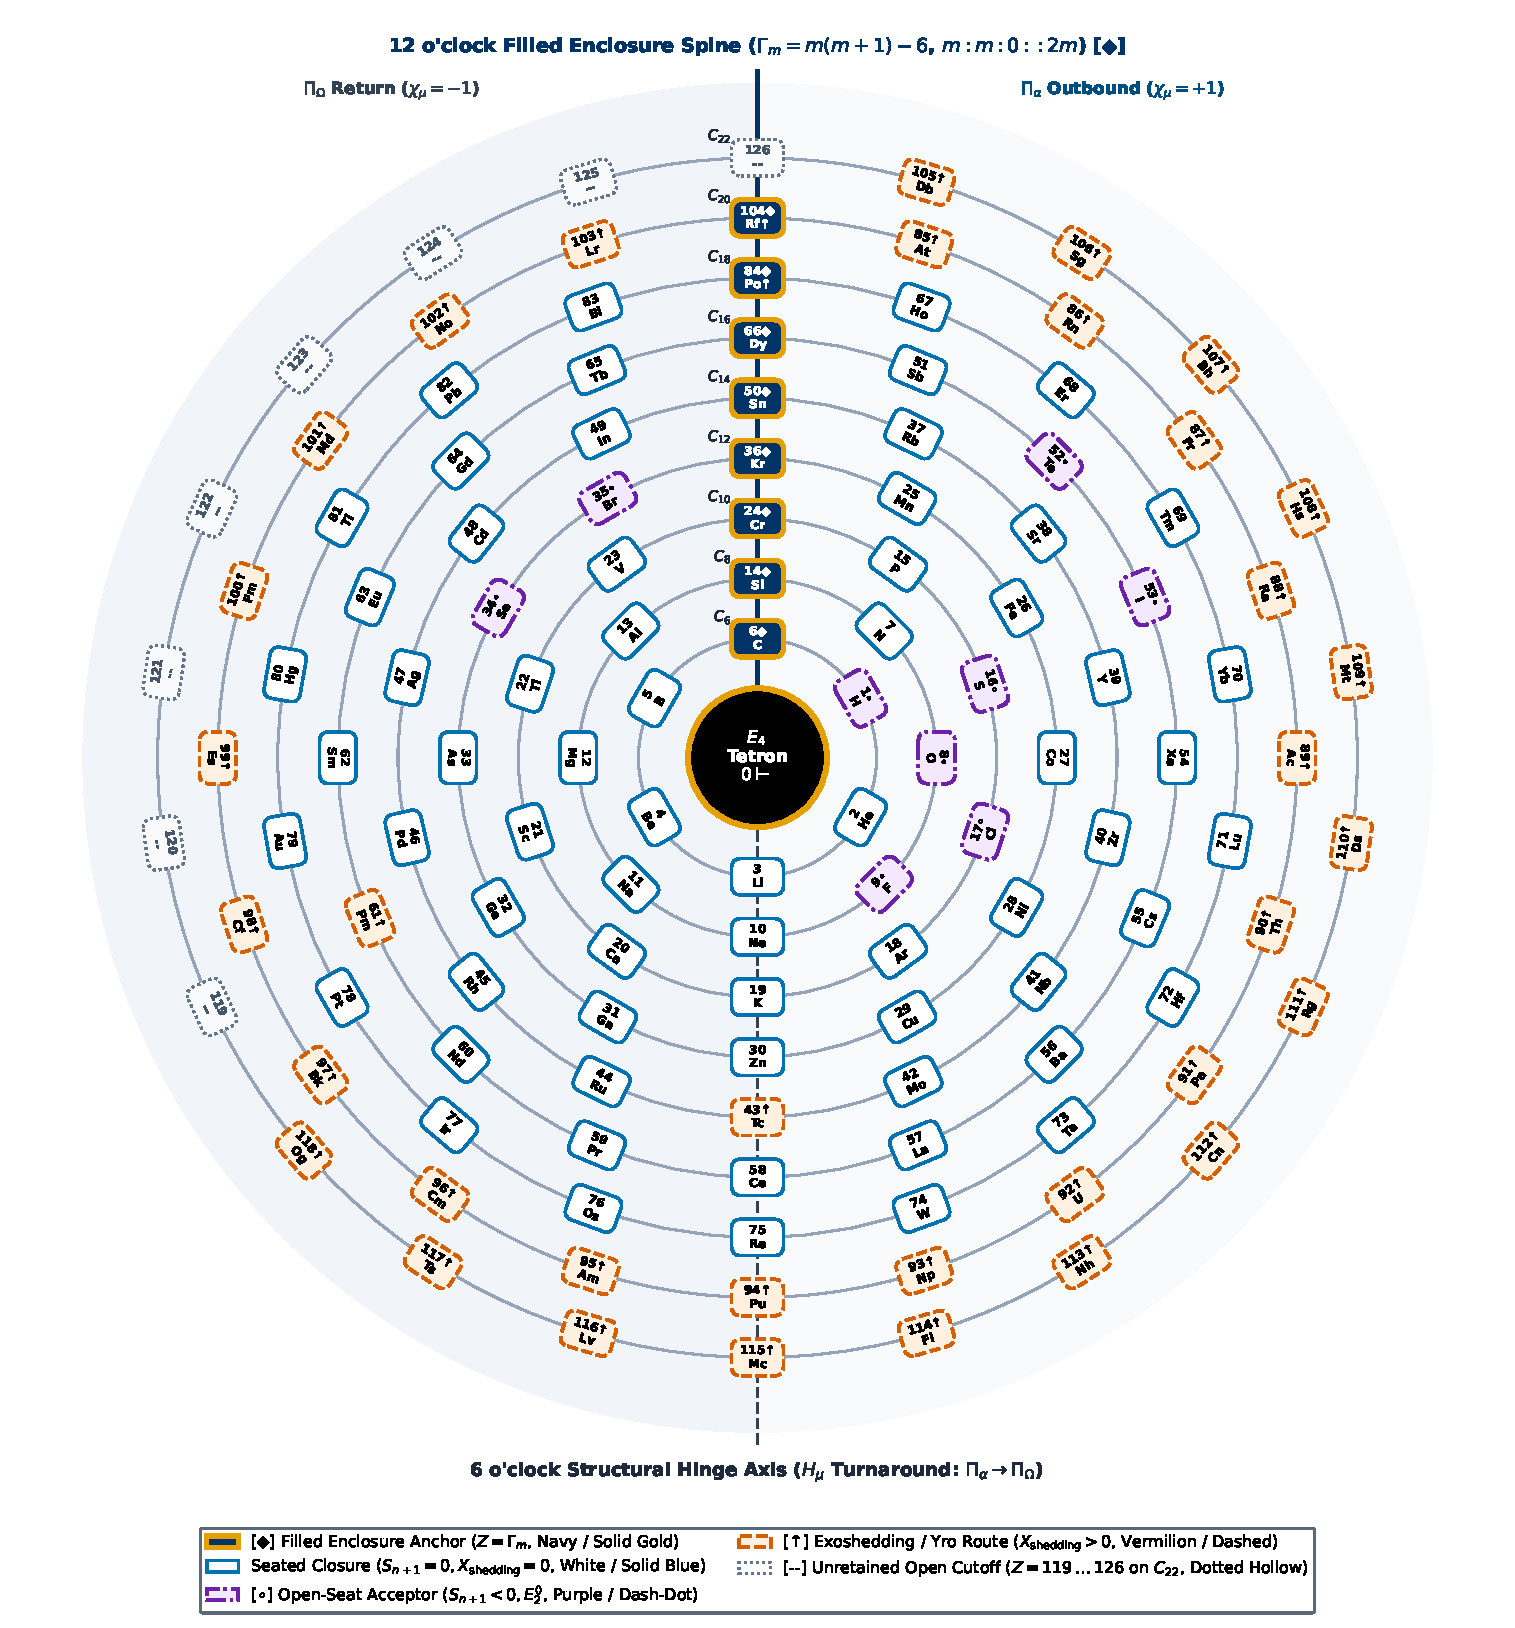
\includegraphics[width=180mm]{figures/aod_matter1_wheel_accessible.pdf}}
\caption{\textbf{Matter I static relational reference.} Nested enclosure membership and repeated branch/hinge/counterbranch roles organize all 118 element labels. The line is a seat-order guide. Positions 119--126 are unfilled reference slots in the declared grouping. Geometry supplies neither physical scale nor an executed network.}
\label{fig:matter1-concentric-wheel}
\end{figure}

% Keep the dedicated chart page before the following derivation.
\clearpage
